%% ----------------------------------------------------------------
%% Thesis.tex -- MAIN FILE (the one that you compile with LaTeX)
%% ---------------------------------------------------------------- 

% Set up the document
\documentclass[a4paper, 11pt, oneside]{Thesis}  % Use the "Thesis" style, based on the ECS Thesis style by Steve Gunn
\graphicspath{Figures/}  % Location of the graphics files (set up for graphics to be in PDF format)

% Include any extra LaTeX packages required
\usepackage[square, numbers, comma, sort&compress]{natbib}  % Use the "Natbib" style for the references in the Bibliography
\usepackage{verbatim}  % Needed for the "comment" environment to make LaTeX comments
\usepackage{vector}  % Allows "\bvec{}" and "\buvec{}" for "blackboard" style bold vectors in maths

\hypersetup{urlcolor=blue, colorlinks=true}  % Colours hyperlinks in blue, but this can be distracting if there are many links.

%% ----------------------------------------------------------------
\begin{document}
\frontmatter      % Begin Roman style (i, ii, iii, iv...) page numbering



%\title{Evaluation of Android Security}
%\author{Saidur Rahman \and Md Ashiqul Mostofa}



\newcommand{\HRule}{\rule{\linewidth}{0.5mm}} % Defines a new command for the horizontal lines, change thickness here

\center % Center everything on the page
 
%----------------------------------------------------------------------------------------
%	HEADING SECTIONS
%----------------------------------------------------------------------------------------
\title{
\textsc{\LARGE Bangladesh University of Engineering and Technology}\\[1.5cm]} % Name of your university/college
%\textsc{\Large Major Heading}\\[0.5cm] % Major heading such as course name
%\textsc{\large Minor Heading}\\[0.5cm] % Minor heading such as course title

%----------------------------------------------------------------------------------------
%	TITLE SECTION
%----------------------------------------------------------------------------------------

\HRule \\[0.4cm]
{ \huge \bfseries Computer Usage and Multimedia Induced Emotion Relationship}\\[0.4cm] % Title of your document
\HRule \\[1.5cm]
 
%----------------------------------------------------------------------------------------
%	AUTHOR SECTION
%----------------------------------------------------------------------------------------

\begin{minipage}{0.4\textwidth}
\begin{flushleft} \large
\emph{AUTHOR:}\\
Rayhan Shikder \\% Your name
0905060
\end{flushleft}
\end{minipage}
~
\begin{minipage}{0.4\textwidth}
\begin{flushright} \large
\emph{SUPERVISOR:} \\
Dr. A.B.M. Alim Al Islam\\% Supervisor's Name
Assistant Professor,\\
Department of CSE, BUET
\end{flushright}
\end{minipage}\\[4cm]

% If you don't want a supervisor, uncomment the two lines below and remove the section above
%\Large \emph{Author:}\\
%John \textsc{Smith}\\[3cm] % Your name

%----------------------------------------------------------------------------------------
%	DATE SECTION
%----------------------------------------------------------------------------------------

{\large \today}\\[3cm] % Date, change the \today to a set date if you want to be precise

%----------------------------------------------------------------------------------------
%	LOGO SECTION
%----------------------------------------------------------------------------------------


\includegraphics[width = 40mm]{Chapters/figures/logo.png}\\[8ex] % Include a department/university logo - this will require the graphicx package


\textsc{Department of Computer Science and Engineering}\\
\textsc{\LARGE Bangladesh University of Engineering and Technology}

\clearpage


% The Abstract Page
\addtotoc{Abstract}  % Add the "Abstract" page entry to the Contents
\abstract{
Devices, capable of detecting human emotion and interacting accordingly is an important part of building intelligent computers. Emotionally-aware systems will be able to make appropriate
decisions about how to interact with the user or adapt their response. There are two main problems with current system approaches for identifying emotions that limit their applicability: they demand additional infrastructures which are often intrusive and require specialized information which are not always available. We experimented on detecting emotion by analyzing the pattern of their keyboard and mouse usage parameters.
 We conducted a field study where we tried to identify users different emotional states, users identity in many different ways by using two types of different classifiers. Our best result shows good result in identifying 3-class emotion, dominant user identity with data from only one emotional state.

}

\clearpage  % Abstract ended, start a new page
%% ----------------------------------------------------------------

\setstretch{1.3}  % Reset the line-spacing to 1.3 for body text (if it has changed)

% The Acknowledgements page, for thanking everyone
\acknowledgements{
\addtocontents{toc}{\vspace{1em}}  % Add a gap in the Contents, for aesthetics

Farzia Afroze, Kazi Zubayer Hasan, Saiyma Sarmin and all the participants of the survey.

}
\clearpage  % End of the Acknowledgements
%% ----------------------------------------------------------------

\pagestyle{fancy}  %The page style headers have been "empty" all this time, now use the "fancy" headers as defined before to bring them back


%% ----------------------------------------------------------------
\lhead{\emph{Contents}}  % Set the left side page header to "Contents"
\tableofcontents  % Write out the Table of Contents

%% ----------------------------------------------------------------
\lhead{\emph{List of Figures}}  % Set the left side page header to "List if Figures"
\listoffigures  % Write out the List of Figures

%% ----------------------------------------------------------------
\lhead{\emph{List of Tables}}  % Set the left side page header to "List of Tables"
\listoftables  % Write out the List of Tables

%% ----------------------------------------------------------------
\setstretch{1.5}  % Set the line spacing to 1.5, this makes the following tables easier to read
\clearpage  % Start a new page
\lhead{\emph{Abbreviations}}  % Set the left side page header to "Abbreviations"
\listofsymbols{ll}  % Include a list of Abbreviations (a table of two columns)
{
% \textbf{Acronym} & \textbf{W}hat (it) \textbf{S}tands \textbf{F}or \\
\textbf{FAR} & \textbf{F}alse \textbf{A}ccept \textbf{R}ate\\
\textbf{FRR} & \textbf{F}alse \textbf{R}eject \textbf{R}ate \\
\textbf{knn} & \textbf{k} \textbf{n}earest \textbf{n}eighbor \\


}

%% ----------------------------------------------------------------
\clearpage  % Start a new page

%% ----------------------------------------------------------------
\mainmatter	  % Begin normal, numeric (1,2,3...) page numbering
\pagestyle{fancy}  % Return the page headers back to the "fancy" style

% Include the chapters of the thesis, as separate files
% Just uncomment the lines as you write the chapters

\chapter{Introduction}
\begin{flushleft}
Emotion is, perhaps, the most critical attribute of living beings that is critical to detect and generate artificially. Its detection always remains a classical well-explored problem.Emotionally-aware systems
would have a rich context from which to make appropriate
decisions about how to interact with the user or adapt their
system response. There exist many approaches for determining human emotions based on facial expression analysis \cite{ioannou}, thermal imaging of faces \cite{kong}, gesture and pose tracking \cite{gunes}, voice intonation \cite{kwon}, etc.We conducted a field study where we collected
participants’ keystrokes, mouse usages and their emotional states via a survey system by inducing emotion through multimedia components.From this data, we extracted important features,
and created classifiers for 10 emotional states. Our top
results include classification of 3-level emotion(positive emotion, negative emotion and neutral emotion), 4-class dominant emotion(amusement, surprise, anger, disgust), dominant user classification etc.
\end{flushleft}














%Introduction

\chapter{Related Work}
\begin{flushleft}
Modeling affective state using typing rhythms draws from
two fields: affective computing and keystroke dynamics.

\subsection{Affective Computing}
Affective computing refers to “computing that relates to,
arises from, or deliberately influences emotions” \cite{picard}. We
are interested in identifying a user’s emotional state, so we
must first consider how emotions are described, and what
other approaches have been used to classify emotion. The
terms affect and emotion are often used interchangeably;
we will use emotional state to refer to the internal dynamics
(cognitive and physiological) that are present during an
emotional episode, and emotional experience as what an
individual perceives of their emotional state \cite{picard}.

\subsubsection{Describing Emotions}
Two main approaches have been used to describe emotions:
categorical and dimensional. The categorical approach
applies specific labels to different emotional states through
language (e.g. sadness, fear, joy) \cite{ekman}. The dimensional
approach \cite{russell} uses two orthogonal axes called arousal and
valence. Arousal is related to the energy of the feeling and
is typically described in terms of low (e.g. sleepiness) to
high (e.g. excitement) arousal. Valence describes the
pleasure (positive) or displeasure (negative) of a feeling.
Labels for different emotional states can be represented in
this two-dimensional space. For example, anger would be a
high-arousal, low-valence state.
\subsubsection{Sensing Emotional State}

Both the categorical and dimensional models of emotion
have been used in prior approaches of identifying emotional
state. Some approaches use features easily discernable by
other humans, such as facial expressions, gestures, vocal
intonation, and language \cite{picard}. For example, face-tracking
software is used to analyze facial expressions gathered from
webcam images to infer users’ affective states  \cite{silva, partala}. This
approach has been extended to use thermal imaging to
identify changes in blood flow patterns of the face that are
synonymous with different facial expressions \cite{khan}.

Other approaches use features that are less discernable to
other humans, but can be measured by specialized
equipment. For example, significant research has been
conducted on measuring physiological changes that occur
in the body during emotional episodes using sensors such as
galvanic skin response, electromyography of the face, and heart activity (see \cite{fairclough} for an overview). In HCI,
researchers have used physiological sensors to measure the
affective state of a user interacting with technology. Results
have been produced by studying users playing video games \cite{mandryk}, navigating web pages \cite{ward}, using video conferencing
software, and using mobile technology \cite{chen}.

The above approaches have two main problems that prevent
their widespread use: the sensing technology is obtrusive,
and requires expensive specialized equipment. For example,
EKG is measured using electrodes attached directly to the
user’s skin. In some cases, the area where the electrodes are
placed needs to be shaved to prevent interference \cite{stern}.
Although research is underway to integrate these sensors
into interaction devices, they are currently intrusive and
their mere presence may alter the user’s emotional state. In
\cite{khan}, a thermal camera is used is measure blood flow to a
user’s face. Although unobtrusive, the equipment is
specialized and not found in typical home or office settings.
To eliminate the need for intrusive and costly equipment,
we propose to determine affective state via typing rhythms.

\subsection{Keystroke Dynamics}

Keystroke dynamics is the study of the unique timing
patterns in an individual’s typing, and typically includes
extracting keystroke timing features such as the duration of
a key press and the time elapsed between key presses.

Much of the previous research in keystroke dynamics has
been in authentication systems, with the premise that, just
as with handwritten signatures, the way that an individual
types can be unique enough to identify them \cite{joyce}. The use
of keystroke dynamics for user authentication has been an
active area of research, producing many studies
 \cite{bergadano, dowland, joyce, monrose }, patents \cite{bender}, and systems \cite{admit}, whereby users
are authenticated by providing the correct user name,
password, and typing rhythm (see \cite{epp} for an overview).
Anecdotal evidence suggests that strong emotional states
can interfere with authentication \cite{monrose}; however, little is
mentioned of this and it is unclear whether the timing
variance associated with these emotional states is similar
between individuals.


Most of the authentication systems \cite{bergadano, joyce, monrose} use fixed-text
models – that is, they use the same static piece of text
(entered during authentication) that the model was trained
on. There have been fewer approaches \cite{dowland, gunetti, monrose} that use
models based on free text (text that is not prescribed to the
user), as they do not perform as well as fixed-text models
\cite{monrose}. The length of the required training text varies between
different studies; some require a few words \cite{bergadano} or full pages
of text \cite{gaines}, which can create better performing models.


Although fixed-text models generally perform better than
free-text models, the potential applications of free-text
models are desirable. Recent work has explored free-text
models for use in continuous verification, where users are
continually monitored to identify masqueraders at any time
(not just during authentication), and have shown potential given enough samples of sufficient length \cite{gunetti}. Free-text
models have even been able to identify individuals typing
in different languages \cite{gunetti2} as long as the two languages
have enough similar valid digraphs. Most free-text studies
require users to enter any ‘valid’ text as sample text \cite{gunetti};
however, in \cite{dowland} keystroke activity was monitored as a
background process during normal computer use. This
method had three benefits: the user was less disturbed by
the collection method, the data was obtained unobtrusively,
and it reduced the cognitive load on the user by avoiding
situations where they must think of something to type.


Classification algorithms for the analysis of keystroke
dynamics for user authentication include neural networks
\cite{brown}, distance measures \cite{joyce, monrose}, decision trees \cite{sheng}, and
other statistical methods \cite{bergadano, dowland, monrose}. Due to the differences in
data collection approaches and classification methods, a
comparison of performance across studies is difficult \cite{bergadano}.

\subsubsection{Keystroke Dynamics and Affective Computing}
There has been very little previous work applying keystroke
dynamics to affective computing.
Zimmerman et al. \cite{zimmermann} describe a method to correlate user
interactions (keyboard and mouse) with affective state.
Affective states were induced using films. Physiological
sensors were used in conjunction with the Self-Assessment
Manikin (SAM) \cite{lang}, a method of subjectively expressing
affective state. The authors found significant differences
between the neutral state and other emotional states, but
were unable to distinguish between the induced states.
Recent work by Vizer et al. \cite{vizer} used keystroke timing
features of free text in conjunction with linguistic features
to identify cognitive and physical stress. They achieved
correct classifications of 62.5% for physical stress and 75%
for cognitive stress (for 2 classes), which they state is
comparable to other affective computing solutions. They
also state that their solutions should be tested with varying
typing abilities and keyboards, with varying physical and
cognitive abilities, and in real-world stressful situations.

 % Background Theory 

\chapter{Motivation behind our work}
Existing emotion detection approaches usually demand additional infrastructures such as webcam, body mounted hardware, etc., which are often intrusive. This approaches also require specialized information such as voice, gestures, facial expression, etc., which are not always available. We propose a novel emotion detection system that detects emotion from widely-used electronic devices demanding no additional infrastructures, and exploiting conventionally available usage data.
\begin{figure}
\centering
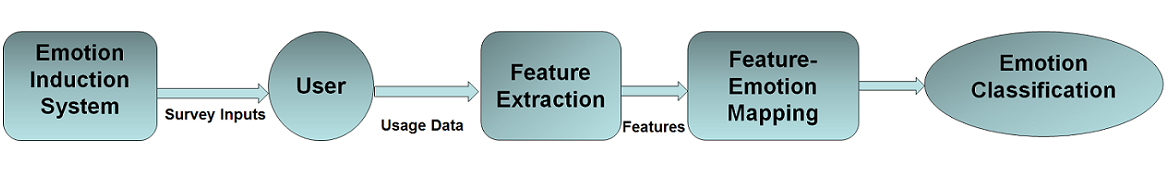
\includegraphics[width=5.25in,clip,keepaspectratio]{Chapters/figures/workingProcedure2.png}
\caption{Our proposed approach for emotion detection}
\label{Optional }
\end{figure}

 % Experimental Setup


\chapter{Emotion Induction}
We used movie clips or short films of around 2 minutes length to induce emotion into users. There were related still pictures and texts also. The videos, still pictures and texts were selected after reviewing by around 10 individuals. All the videos, still pictures and texts were presented among 10 persons and they were asked to tell their emotional states after watching each video, still picture and text. We developed a induction and survey system for our study, where we presented these selected videos, images and texts to induce certain emotions and then prompted the user with some related questions. To answer the questions user have to use both keyboard and mouse of the computer.
 % Experiment 1


\chapter{Tracking usage parameters}
While answering the question, users certain usage attributes are logged automatically in every 5 seconds. There are 17 attributes that are logged. The attributes are average mouse left click, average mouse right click, average mouse double click, average mouse scroll, average cursor x-distance, average cursor y-distance, average key down to up time, average key up to down time, average key down to down time, average regular key press, average enter key press, average arrow key press, average backspace key press, average function key press etc. We also collected some meta data from the user. These are the name, age, occupation and birth year of the survey participant.

\begin{figure}
\centering
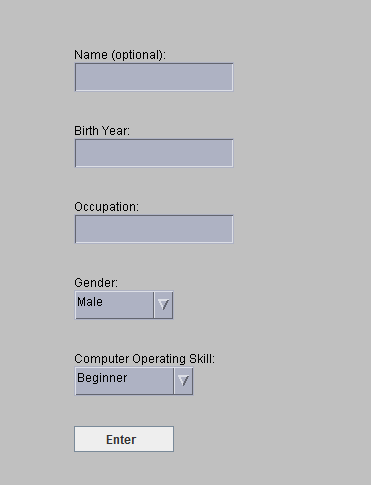
\includegraphics[width=3in,clip,keepaspectratio]{Chapters/figures/startPageSurvey.png}
\caption{Start page of the survey}
\label{Optional }
\end{figure}

\begin{figure}
\centering
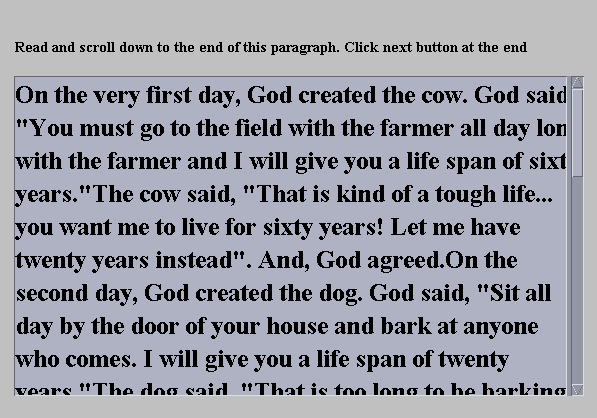
\includegraphics[width=2.5in,clip,keepaspectratio]{Chapters/figures/scrollText.png}
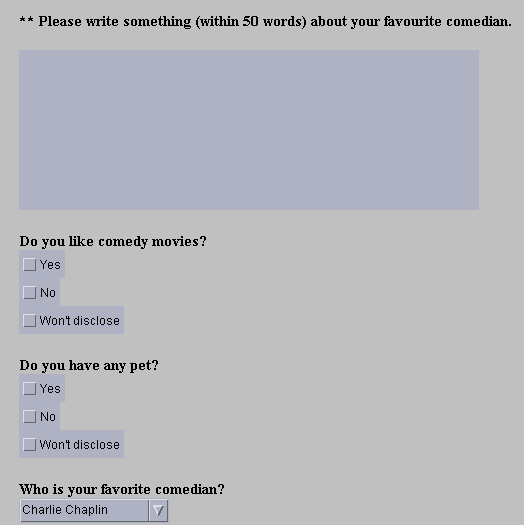
\includegraphics[width=2.5in,clip,keepaspectratio]{Chapters/figures/survey.png}
\caption{Text and various questions to capture scrolling and other usage attributes}
\label{Optional2 }
\end{figure}

 % Experiment 2


\chapter{Emotion Usage Relationship}
should write something here




\subsection{Demography of participants}
There were a total of 26 participants. 19 of them were male and 7 were female. Most of them were students and some are from other occupations. 
\begin{figure}
\centering
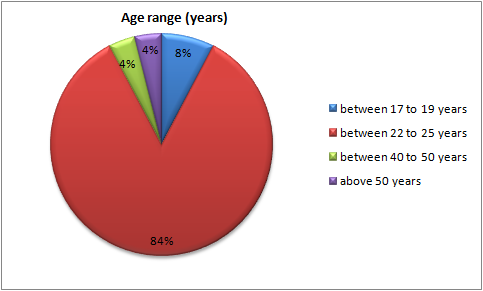
\includegraphics[width=1.75in,clip,keepaspectratio]{Chapters/figures/ageChart3}
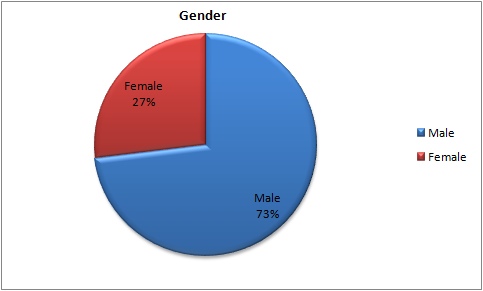
\includegraphics[width=1.75in,clip,keepaspectratio]{Chapters/figures/gender3}
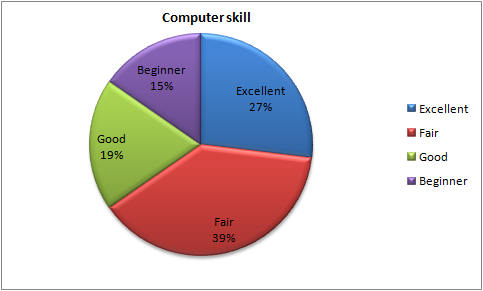
\includegraphics[width=1.75in,clip,keepaspectratio]{Chapters/figures/skill}
\caption{Category of users based on age range, gender, and computer operating skill}
\label{Optional 3 }
\end{figure}




\subsection{Classification methods}
\subsubsection{Bounded k-means clustering}
In these approach we used a variant of k-means clustering approach, where we put a constraint on the cluster size. The cluster size was varied to find out the optimal cluster size so that the total false acceptance and false rejection are minimized. The size was varied with percentages of mean and standard deviation.

\begin{figure}
\centering
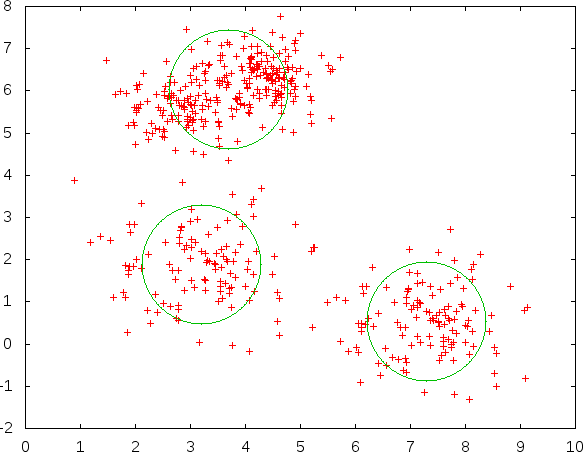
\includegraphics[width=3in,clip,keepaspectratio]{Chapters/figures/boundeKmeans}
\caption{bounded k-means clustering}
\label{Optional 4 }
\end{figure}

\subsubsection{k-nearest neighbor}
We used this well known classification method where a test point is classified by examining its neighbor points. We varied both the number of neighbors and the number of attributes.

\subsection{Identification of emotional states}
At first we tried to classify human emotions based on the usage attributes we captured in each step of the survey process. Every captured data is like the following format:
Att1, att2, att3, ………, emotion label, user label.

\subsubsection{10 classes of emotions}
We tried to classify 10 different emotional states. These are amusement, happiness, inspiration, surprise, sadness, sympathy, anger, disgust, fear and neutral emotion.
We tried two different classification approaches: bounded k-means clustering and k-nearest neighbor method.
\begin{center}
\begin{table}

\centering
\begin{tabular}{ |c|c|c| } 
 \hline
 method & false accept rate & false reject rate \\ 
 \hline
 bounded k-means & 0.43 & 0.34 \\ 
 knn & 0.76 & 0.0 \\ 
 \hline
\end{tabular}

\caption{bounded k-means and knn for 10 class emotion classification}
\label{table:1}
\end{table}
\end{center}

\begin{figure}
\centering
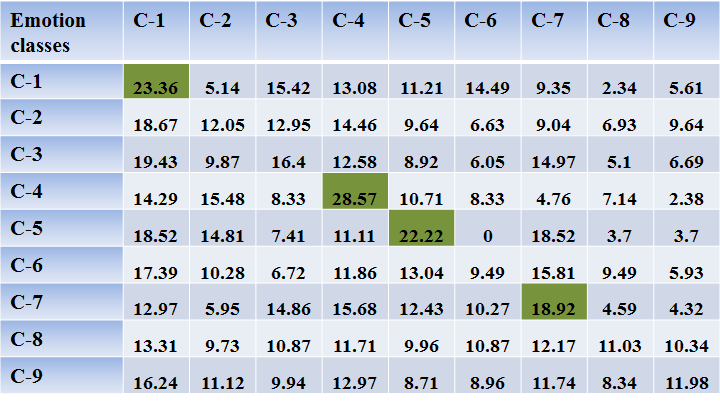
\includegraphics[width=4.25in,clip,keepaspectratio]{Chapters/figures/emotionMatrix}
\caption{Matrix of domination for 9-emotion classes(without the neutral emotion)}
\label{Optional 6}
\end{figure}


\begin{figure}
\centering
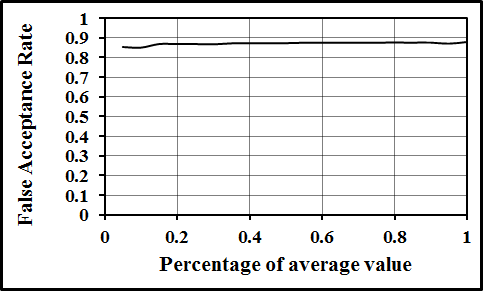
\includegraphics[width=2.5in,clip,keepaspectratio]{Chapters/figures/Emotion/10class/fA}
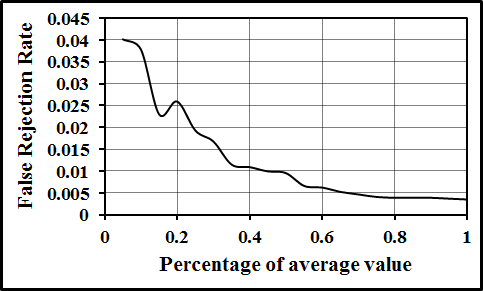
\includegraphics[width=2.5in,clip,keepaspectratio]{Chapters/figures/Emotion/10class/fR}
\caption{percentage of average vs false accept rate and false reject rate in bounded k-means for 10 class emotion classification}
\label{Optional 5}
\end{figure}

\begin{figure}
\centering
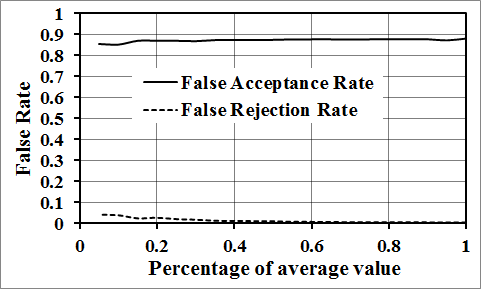
\includegraphics[width=4.25in,clip,keepaspectratio]{Chapters/figures/Emotion/10class/fAfR}
\caption{percentage of average vs false accept rate and false reject rate in bounded k-means for 10 class emotion classification}
\label{Optional 5}
\vskip -1cm
\end{figure}



\subsubsection{3 classes of emotions}
We grouped the 10 classes into 3 groups. The positive emotions such as amusement, happiness, inspiration and surprise were grouped into one class. The negative emotions such as sadness, sympathy, anger, disgust and fear were grouped into one class. Neutral emotion was considered as the third class.


\begin{center}
\begin{table}

\centering
\begin{tabular}{ |c|c|c| } 
 \hline
 method & false accept rate & false reject rate \\ 
 \hline
 bounded k-means & 0.25 & 0.17 \\ 
 knn & 0.47 & 0.0 \\ 
 \hline
\end{tabular}

\caption{bounded k-means and knn for 3 class emotion classification}
\label{table:2}
\end{table}
\end{center}


\begin{figure}
\centering
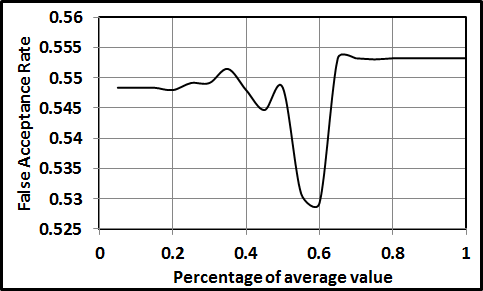
\includegraphics[width=4.25in,clip,keepaspectratio]{Chapters/figures/Emotion/3class/fA}
\caption{percentage of average vs false accept rate and false reject rate in bounded k-means for 3 class emotion classification}
\label{Optional 6}
\end{figure}


\clearpage
\subsubsection{Dominant classes of emotions}

\begin{center}

\begin{table}

\centering
\begin{tabular}{ |c|c|c|c|c| } 
 \hline
 classes & Amusement & Surprise & Sadness & Anger \\
\hline
Amusement & 36.31 &  25.34 &  16.75 &  21.60 \\ 
Surprise & 28.83 &  31.08 &  21.62 &  18.47 \\
Sadness & 27.60 &  25.04 &  22.78  & 24.59 \\ 
Anger & 24.04 &  22.70 &  18.43 &  34.83 \\

\hline
\end{tabular}

\caption{matrix of cluster with only dominant emotions}
\label{table:4}
\end{table}
\end{center}

\begin{figure}
\centering
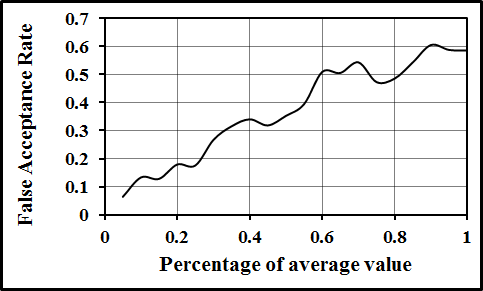
\includegraphics[width=2.5in,clip,keepaspectratio]{Chapters/figures/Emotion/dominant/fA}
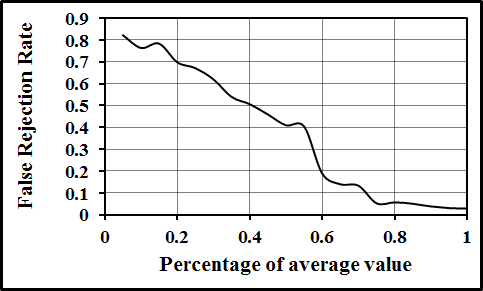
\includegraphics[width=2.5in,clip,keepaspectratio]{Chapters/figures/Emotion/dominant/fR}

\caption{percentage of average vs false accept rate and false reject rate in bounded k-means for dominant emotion classfication}
\label{Optional 6}
\end{figure}

\begin{figure}
\centering
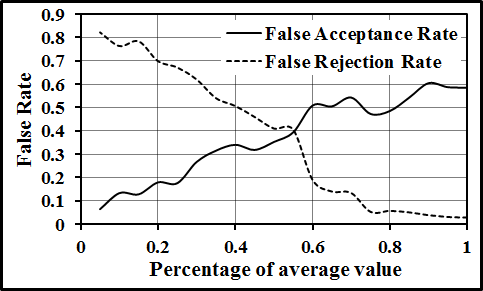
\includegraphics[width=4.25in,clip,keepaspectratio]{Chapters/figures/Emotion/dominant/fAfR}
\caption{percentage of average vs both false accept rate and false reject rate in bounded k-means for dominant emotion classfication}
\label{Optional 6}
\end{figure}


From the unsupervised bounded k-means clustering of 10 emotions. We found 10 different clusters, but this clusters were not dominated by only one class of emotion. Rather we found that there are some emotions which dominates not only in his own cluster but also in the clusters of others. While trying to classify these dominant clusters only we found some improvement. The experimental results are as followed from bounded k-means clustering and k-nearest neighbor classification:


\clearpage
\subsubsection{Less Dominant classes of emotions}
From the cluster matrix we can identify the clusters(emotions) which has less influence over their own clusters and others clusters. When we tried to classify these less dominant emotions, we found the following results:


\begin{table}

\centering
\begin{tabular}{ |c|c|c|c|c|c| } 
 \hline
 classes & c-1 & c-2 & c-3 & c-4 & c-5\\
\hline
c-1 & 26.32 & 26.32 & 16.67 & 12.72 & 17.98 \\
c-2 & 18.69 & 38.13 & 17.93 & 11.62 & 13.64 \\ 
c-3 & 21.31 & 21.31 & 26.23 & 17.49 & 13.66 \\
c-4  & 18.34 & 20.92 & 20.63 & 20.77 & 19.34 \\
c-5  & 22.09 & 19.75 & 17.79 & 16.56 & 23.80 \\

\hline
\end{tabular}

\caption{matrix of cluster with less dominant emotions}
\label{table:5}
\end{table}


\begin{figure}
\centering
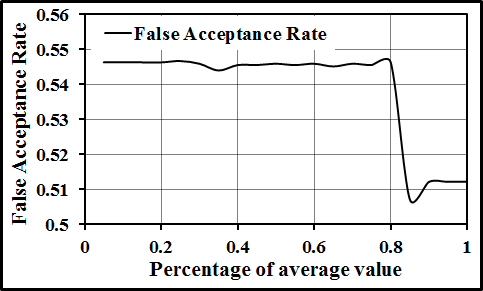
\includegraphics[width=2.5in,clip,keepaspectratio]{Chapters/figures/Emotion/lessDominant/fA}
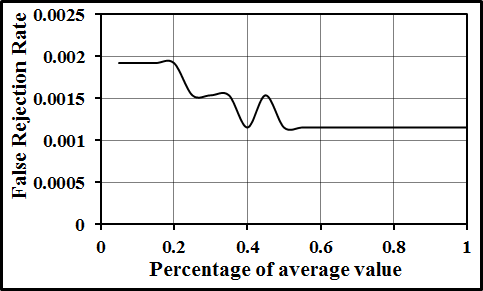
\includegraphics[width=2.5in,clip,keepaspectratio]{Chapters/figures/Emotion/lessDominant/fR}
\caption{percentage of average vs false accept rate and false reject rate in bounded k-means for less dominant emotion classification}
\label{Optional 6}
\end{figure}

\begin{figure}
\centering
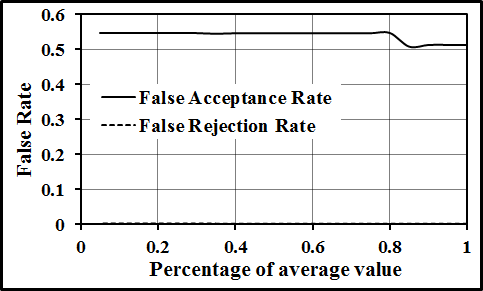
\includegraphics[width=4.25in,clip,keepaspectratio]{Chapters/figures/Emotion/lessDominant/fAfR}
\caption{percentage of average vs false accept rate and false reject rate in bounded k-means for less dominant emotion classification}
\label{Optional 6}
\end{figure}



\clearpage
\subsection{User classification}
\subsubsection{All user classification}
What about classifying a user based on his usage attributes. In this case we considered the data without any normalization. At first we tried to cluster the data with our unsupervised clustering approach (bounded k-means clustering). But we found it difficult to successfully identify users based on their usage attributes.
The experimental results are as follows


\subsubsection{Dominant user classification}
From matrix of users clusters, we found that some of the users heavily dominates others clusters. So we made an attempt to classify these dominant users. The results we found was much better than the general case. The results are illustrated below:

\begin{figure}
\centering
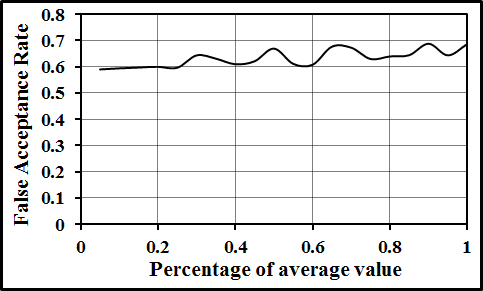
\includegraphics[width=2.5in,clip,keepaspectratio]{Chapters/figures/User/dominant/fA}
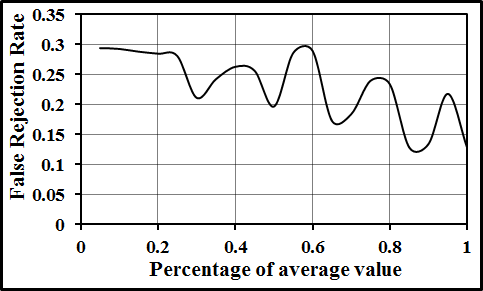
\includegraphics[width=2.5in,clip,keepaspectratio]{Chapters/figures/User/dominant/fR}
\caption{percentage of average vs false accept rate and false reject rate in bounded k-means for dominant user classification}
\label{Optional 6}
\end{figure}


\begin{figure}
\centering
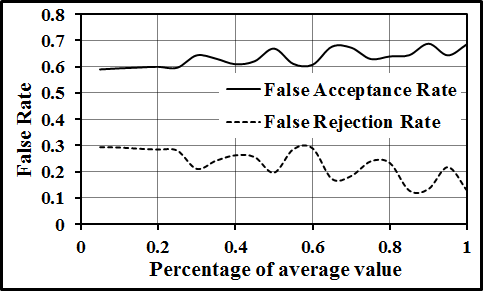
\includegraphics[width=4.25in,clip,keepaspectratio]{Chapters/figures/User/dominant/fAfR}
\caption{percentage of average vs both false acceptance rate and false rejection rate in bounded k-means for dominant user classification}
\label{Optional 6}
\end{figure}


\clearpage
\subsubsection{Dominant user classification with neutral emotion only}
From matrix of users clusters, we found that some of the users heavily dominates others clusters. So we made an attempt to classify these dominant users. The results we found was much better than the general case. The results are illustrated below:

\begin{figure}
\centering
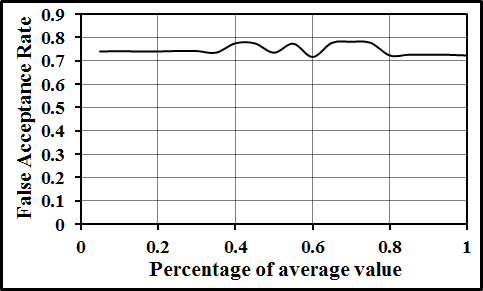
\includegraphics[width=2.5in,clip,keepaspectratio]{Chapters/figures/User/dominantWithNeutral/fA}
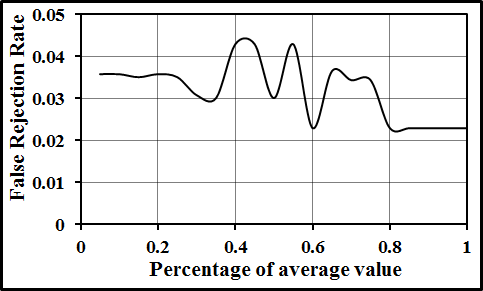
\includegraphics[width=2.5in,clip,keepaspectratio]{Chapters/figures/User/dominantWithNeutral/fR}
\caption{percentage of average vs false accept rate and false reject rate in bounded k-means for dominant user classification with neutral data only}
\label{Optional 6}
\end{figure}


\begin{figure}
\centering
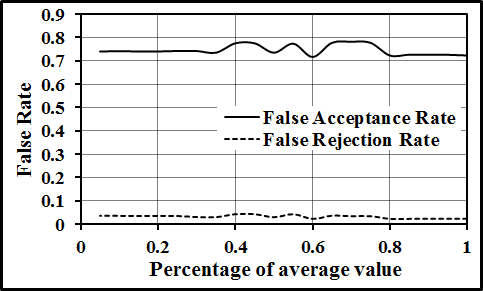
\includegraphics[width=4.25in,clip,keepaspectratio]{Chapters/figures/User/dominantWithNeutral/fAfR}

\caption{percentage of average vs false accept rate and false reject rate in bounded k-means for dominant user classification with neutral data only}
\label{Optional 6}
\end{figure}

\clearpage
\subsubsection{Less Dominant user classification with neutral emotion only}
From matrix of users clusters, we found that some of the users heavily dominates others clusters. So we made an attempt to classify these dominant users. The results we found was much better than the general case. The results are illustrated in figure 6.16.

\begin{figure}
\centering
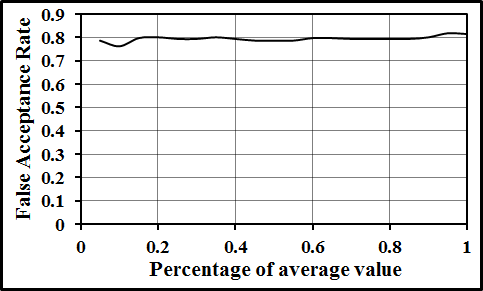
\includegraphics[width=2.5in,clip,keepaspectratio]{Chapters/figures/User/lessDominantWithNeutral/fA}
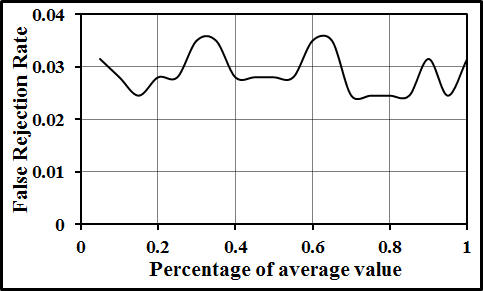
\includegraphics[width=2.5in,clip,keepaspectratio]{Chapters/figures/User/lessDominantWithNeutral/fR}
\caption{percentage of average vs false accept rate and false reject rate in bounded k-means for less dominant user classification with only neutral emotion's value}
\label{Optional 6}
\end{figure}

\begin{figure}
\centering
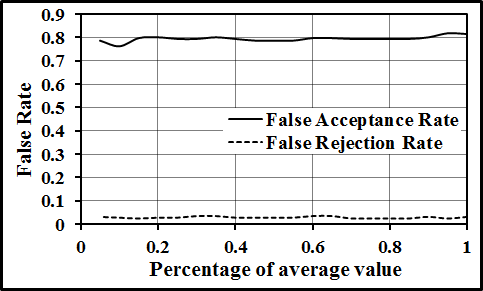
\includegraphics[width=4.25in,clip,keepaspectratio]{Chapters/figures/User/lessDominantWithNeutral/fAfR}
\caption{percentage of average vs false accept rate and false reject rate in bounded k-means for less dominant user classification with only neutral emotion's value}
\label{Optional 6}
\end{figure}




% Balancing columns in a ref list is a bit of a pain because you
% either use a hack like flushend or balance, or manually insert
% a column break.  http://www.tex.ac.uk/cgi-bin/texfaq2html?label=balance
% multicols doesn't work because we're already in two-column mode,
% and flushend isn't awesome, so I choose balance.  See this
% for more info: http://cs.brown.edu/system/software/latex/doc/balance.pdf
%
% Note that in a perfect world balance wants to be in the first
% column of the last page.
%
% If balance doesn't work for you, you can remove that and
% hard-code a column break into the bbl file right before you
% submit:
%
% http://stackoverflow.com/questions/2149854/how-to-manually-equalize-columns-
% in-an-ieee-paper-if-using-bibtex
%
% Or, just remove \balance and give up on balancing the last page.
%

 % Results and Discussion

\chapter{Conclusion}

Devices, capable of detecting human emotion and interacting accordingly is an important part of building intelligent computers. An emotionally aware system will be much user friendly, and less frustrating for the users as it will be able to make appropriate decisions about how to interact with the user or adapt their response. There are two main problems with current system approaches for identifying emotions that limit their applicability: they demand additional infrastructures which are often intrusive and require specialized information which are not always available. We experimented on detecting emotion by analyzing the pattern of their keyboard and mouse usage parameters. In our study, we tried to identify users different emotional states, users identity in many different ways by using bounded k-means clustering and k-nearest neighbor approach. Our best result shows good result in identifying 3-class emotion, dominant user identity with data from only one emotional state.
\end{flushleft} % Conclusion

%% ----------------------------------------------------------------
% Now begin the Appendices, including them as separate files

\addtocontents{toc}{\vspace{2em}} % Add a gap in the Contents, for aesthetics

%\appendix % Cue to tell LaTeX that the following 'chapters' are Appendices

%\chapter{An Appendix}

Lorem ipsum dolor sit amet, consectetur adipiscing elit. Vivamus at pulvinar nisi. Phasellus hendrerit, diam placerat interdum iaculis, mauris justo cursus risus, in viverra purus eros at ligula. Ut metus justo, consequat a tristique posuere, laoreet nec nibh. Etiam et scelerisque mauris. Phasellus vel massa magna. Ut non neque id tortor pharetra bibendum vitae sit amet nisi. Duis nec quam quam, sed euismod justo. Pellentesque eu tellus vitae ante tempus malesuada. Nunc accumsan, quam in congue consequat, lectus lectus dapibus erat, id aliquet urna neque at massa. Nulla facilisi. Morbi ullamcorper eleifend posuere. Donec libero leo, faucibus nec bibendum at, mattis et urna. Proin consectetur, nunc ut imperdiet lobortis, magna neque tincidunt lectus, id iaculis nisi justo id nibh. Pellentesque vel sem in erat vulputate faucibus molestie ut lorem.

Quisque tristique urna in lorem laoreet at laoreet quam congue. Donec dolor turpis, blandit non imperdiet aliquet, blandit et felis. In lorem nisi, pretium sit amet vestibulum sed, tempus et sem. Proin non ante turpis. Nulla imperdiet fringilla convallis. Vivamus vel bibendum nisl. Pellentesque justo lectus, molestie vel luctus sed, lobortis in libero. Nulla facilisi. Aliquam erat volutpat. Suspendisse vitae nunc nunc. Sed aliquet est suscipit sapien rhoncus non adipiscing nibh consequat. Aliquam metus urna, faucibus eu vulputate non, luctus eu justo.

Donec urna leo, vulputate vitae porta eu, vehicula blandit libero. Phasellus eget massa et leo condimentum mollis. Nullam molestie, justo at pellentesque vulputate, sapien velit ornare diam, nec gravida lacus augue non diam. Integer mattis lacus id libero ultrices sit amet mollis neque molestie. Integer ut leo eget mi volutpat congue. Vivamus sodales, turpis id venenatis placerat, tellus purus adipiscing magna, eu aliquam nibh dolor id nibh. Pellentesque habitant morbi tristique senectus et netus et malesuada fames ac turpis egestas. Sed cursus convallis quam nec vehicula. Sed vulputate neque eget odio fringilla ac sodales urna feugiat.

Phasellus nisi quam, volutpat non ullamcorper eget, congue fringilla leo. Cras et erat et nibh placerat commodo id ornare est. Nulla facilisi. Aenean pulvinar scelerisque eros eget interdum. Nunc pulvinar magna ut felis varius in hendrerit dolor accumsan. Nunc pellentesque magna quis magna bibendum non laoreet erat tincidunt. Nulla facilisi.

Duis eget massa sem, gravida interdum ipsum. Nulla nunc nisl, hendrerit sit amet commodo vel, varius id tellus. Lorem ipsum dolor sit amet, consectetur adipiscing elit. Nunc ac dolor est. Suspendisse ultrices tincidunt metus eget accumsan. Nullam facilisis, justo vitae convallis sollicitudin, eros augue malesuada metus, nec sagittis diam nibh ut sapien. Duis blandit lectus vitae lorem aliquam nec euismod nisi volutpat. Vestibulum ornare dictum tortor, at faucibus justo tempor non. Nulla facilisi. Cras non massa nunc, eget euismod purus. Nunc metus ipsum, euismod a consectetur vel, hendrerit nec nunc.	% Appendix Title

%\input{Appendices/AppendixB} % Appendix Title

%\input{Appendices/AppendixC} % Appendix Title

\addtocontents{toc}{\vspace{2em}}  % Add a gap in the Contents, for aesthetics
\backmatter

%% ----------------------------------------------------------------
\label{Bibliography}
\lhead{\emph{Bibliography}}  % Change the left side page header to "Bibliography"

\begin{thebibliography}{9}



\bibitem{ioannou} 
S. Ioannou, A. Raouzaiou, V. Tzouvaras, T. Mailis, K. Karpouzis and S. Kollias: "Emotion Recognition through Facial Expression Analysis Based on a Neurofuzzy Method",
\textit{ Neural Networks, }
vol. 18, pp. 423-435, 2005.



\bibitem{kong} 
 S.G. Kong, J. Heo, B. Abidi, J. Paik and M. Abidi: "Recent advances in visual and infrared face recognition—a review"
 \textit{ Computer Vision and Image Understanding,}
 vol. 97, no. 1, pp. 103-135, Jan. 2005.
 
 

\bibitem{gunes} 
H. Gunes and M. Pantic, \& ldquo, “Dimensional Emotion Prediction from Spontaneous Head Gestures for Interaction with Sensitive Artificial Listeners”,
\textit{ Proc. Int',l Conf. Intelligent  
     Virtual Agents,}
pp. 371-377, 2010. 

\bibitem{kwon} 
O. W. Kwon, K. Chan, J. Hao, and T. W. Lee: “Emotion recognition by speech signals,” In Proc. EUROSPEECH, 2003.


\bibitem{picard} 
Picard, R.W. 
\textit{Affective Computing.}
 MIT Press, Cambridge, 2007.
 
\bibitem{ekman} 
Ekman, P. 
\textit{Basic Emotions.}
John Wiley and Sons, Ltd, 2005.

\bibitem{russell} 
Russell, J. Core affect and the psychological
construction of emotion. 
\textit{ Psychological Review 110,}
 1
(2003), 145-172.

\bibitem{silva} 
De Silva, L. and Suen Chun, H. Real-time facial
feature extraction and emotion recognition.
\textit{ Infor.,
Comm., and Sig. Proc. 2003 and the 4th Pac. Rim
Conf. on Multimedia,}
(2003).

\bibitem{khan} 
Khan, M.M., Ingleby, M., and Ward, R.D. Automated
facial expression classification and affect interpretation
using infrared measurement of facial skin temperature
variations.
\textit{ ACM Trans. Auton. Adapt. Syst. 1,}1 (2006),
91-113.


\bibitem{partala} 
Partala, T., Surakka, V., and Vanhala, T. Real-time
estimation of emotional experiences from facial
expressions.
\textit{ Interact. Comput. 18,}2 (2006), 208-226.


\bibitem{fairclough} 
Fairclough, S. Fundamentals of physiological
computing.
\textit{ Inter. with Comp. 21,}1-2 (2009), 133-145.


\bibitem{mandryk} 
Mandryk, R.L. and Atkins, M.S. A fuzzy physiological
approach for continuously modeling emotion during
interaction with play technologies.
\textit{ Int. J. Hum.-
Comput. Stud. 65,} 4 (2007), 329-347.


\bibitem{ward} 
Ward, R.D. and Marsden, P.H. Physiological responses
to different web page designs.
\textit{ Int. J. Hum.-Comput.
Stud. 59, } 1-2 (2003), 199-212.


\bibitem{chen} 
Chen, D. and Vertegaal, R. Using mental load for
managing interruptions in physiologically attentive
user interfaces.
\textit{ CHI '04 ext. abst. on Human fac. in
comp. systems, } ACM (2004), 1513-1516.


\bibitem{stern} 
Stern, R.M., Ray, W.J., and Quigley, K.S.
\textit{ Psychophysiological recording. } Oxford University
Press, New York, 2001.


\bibitem{joyce} 
Joyce, R. and Gupta, G. Identity authentication based
on keystroke latencies.
\textit{ Commun. ACM 33, } 2 (1990),
168-176.

\bibitem{dowland} 
Dowland, P. and Furnell, S. A Long-term trial of
keystroke profiling using digraph, trigraph, and
keyword latencies. In
\textit{ IFIP Intern. Fed. for Infor.
Processing. } Springer Boston, 2004, 275-289.

\bibitem{monrose} 
Monrose, F. and Rubin, A.D. Keystroke dynamics as a biometric for authentication.
\textit{ Future Gener. Comput.
Syst. 16, } 4 (2000), 351-359.


\bibitem{bender} 
Bender, S. and Postley, H. Key sequence rhythm
recognition system and method. .

\bibitem{admit} 
Admit One Security.
\textit{ AdmitOneSecurity. } http://www.admitonesecurity.com.


\bibitem{epp} 
Epp, C. Identifying emotional states through keystroke
dynamics. 2010.http://library2.usask.ca/theses/available/etd-08312010-
131027/.


\bibitem{gunetti} 
Gunetti, D. and Picardi, C. Keystroke analysis of free
text.
\textit{ ACM Trans. Inf. Syst. Secur. 8, } 3 (2005), 312-347.


\bibitem{bergadano} 
Bergadano, F., Gunetti, D., and Picardi, C. User
authentication through keystroke dynamics.
\textit{ ACM
Trans. Inf. Syst. Secur. 5, } 4 (2002), 367-397.


\bibitem{gaines} 
Gaines, R., Lisowski, W., Press, S., and Shapiro, N.
Authentication by keystroke timing: some preliminary
results. 1980.


\bibitem{gunetti2} 
Gunetti, D., Picardi, C., and Ruffo, G. Keystroke
analysis of different languages: a case study. In 
\textit{ Lecture Notes in Computer Science. } Springer Berline /
Heidelberg, 2005, 133-144.


\bibitem{brown} 
Brown, M. and Rogers, S.J. User identification via
keystroke characteristics of typed names using neural networks.
\textit{ Int. J. Man-Mach. Stud. 39, } 6 (1993), 999-1014.

\bibitem{sheng} 
Sheng, Y., Phoha, V., and Rovnyak, S. A parallel
decision tree-based method for user authentication
based on keystroke patterns.
\textit{ IEEE Transactions on
Systems, Man, and Cybernetics 35, } 4 (2005), 826-833.


\bibitem{lang} 
Lang, P. Behavioral treatment and bio-behavioral
assessment: computer applications.
\textit{ Technology in
mental health care delivery systems, } (1980), 119-137.



\bibitem{zimmermann} 
Zimmermann, P., Guttormsen, S., Danuser, B., and
Gomez, P. Affective computing - a rationale for
measuring mood with mouse and keyboard.
\textit{ Inter. J. of
Occ. Saf. and Ergo. 9, } 4 (2003), 539-551.



\bibitem{vizer} 
Vizer, L.M., Zhou, L., and Sears, A. Automated stress
detection using keystroke and linguistic features: An
exploratory study.
\textit{ Int. J. Hum.-Comput. Stud. 67, } 10
(2009), 870-886.



\end{thebibliography}

\end{document}  % The End
%% ----------------------------------------------------------------